\documentclass[]{article}
\usepackage[T1]{fontenc}
\usepackage{lmodern}
\usepackage{amssymb,amsmath}
\usepackage{ifxetex,ifluatex}
\usepackage{fixltx2e} % provides \textsubscript
\usepackage[letterpaper, total={6.5in, 8in}, top=1.75in]{geometry}

% use microtype if available
\IfFileExists{microtype.sty}{\usepackage{microtype}}{}
% use upquote if available, for straight quotes in verbatim environments
\IfFileExists{upquote.sty}{\usepackage{upquote}}{}

\usepackage{fontspec}
\usepackage{xltxtra,xunicode}
\defaultfontfeatures{Mapping=tex-text,Scale=MatchLowercase}

\setmainfont{DINPro}
\setsansfont{DejaVu Sans}
\setmonofont[Mapping=tex-ansi]{DejaVu Sans Mono}

\pagenumbering{arabic}

% Chapters start new pages.
\usepackage{titlesec}
\newcommand{\sectionbreak}{\clearpage\thispagestyle{plain}}

\usepackage{listings}
\usepackage{longtable}

\usepackage{tikz}
\usetikzlibrary{calc}
\usepackage{graphicx}
\usepackage[setpagesize=false, % page size defined by xetex
            unicode=false, % unicode breaks when used with xetex
            xetex]{hyperref}

\usepackage{background}
\backgroundsetup{
  scale=1,
  angle=0,
  opacity=1,
  color=black,
  contents={
    \begin{tikzpicture}[remember picture,overlay]
      \node at ([xshift=-1.8in,yshift=-1.0in] current page.north east)
      {
        
\includegraphics[width=2.2in]{clearpath-logo.pdf}
      }; % logo goes here
    \end{tikzpicture}
  }
}

\setlength{\parindent}{0pt}
\setlength{\parskip}{6pt plus 2pt minus 1pt}
\setlength{\emergencystretch}{3em}  % prevent overfull lines

\begin{document}

\thispagestyle{empty}
\begin{tikzpicture}[remember picture,overlay]
\node[anchor=north west,inner sep=0pt] at ($(current page.north west)+(0cm,0cm)$) {
  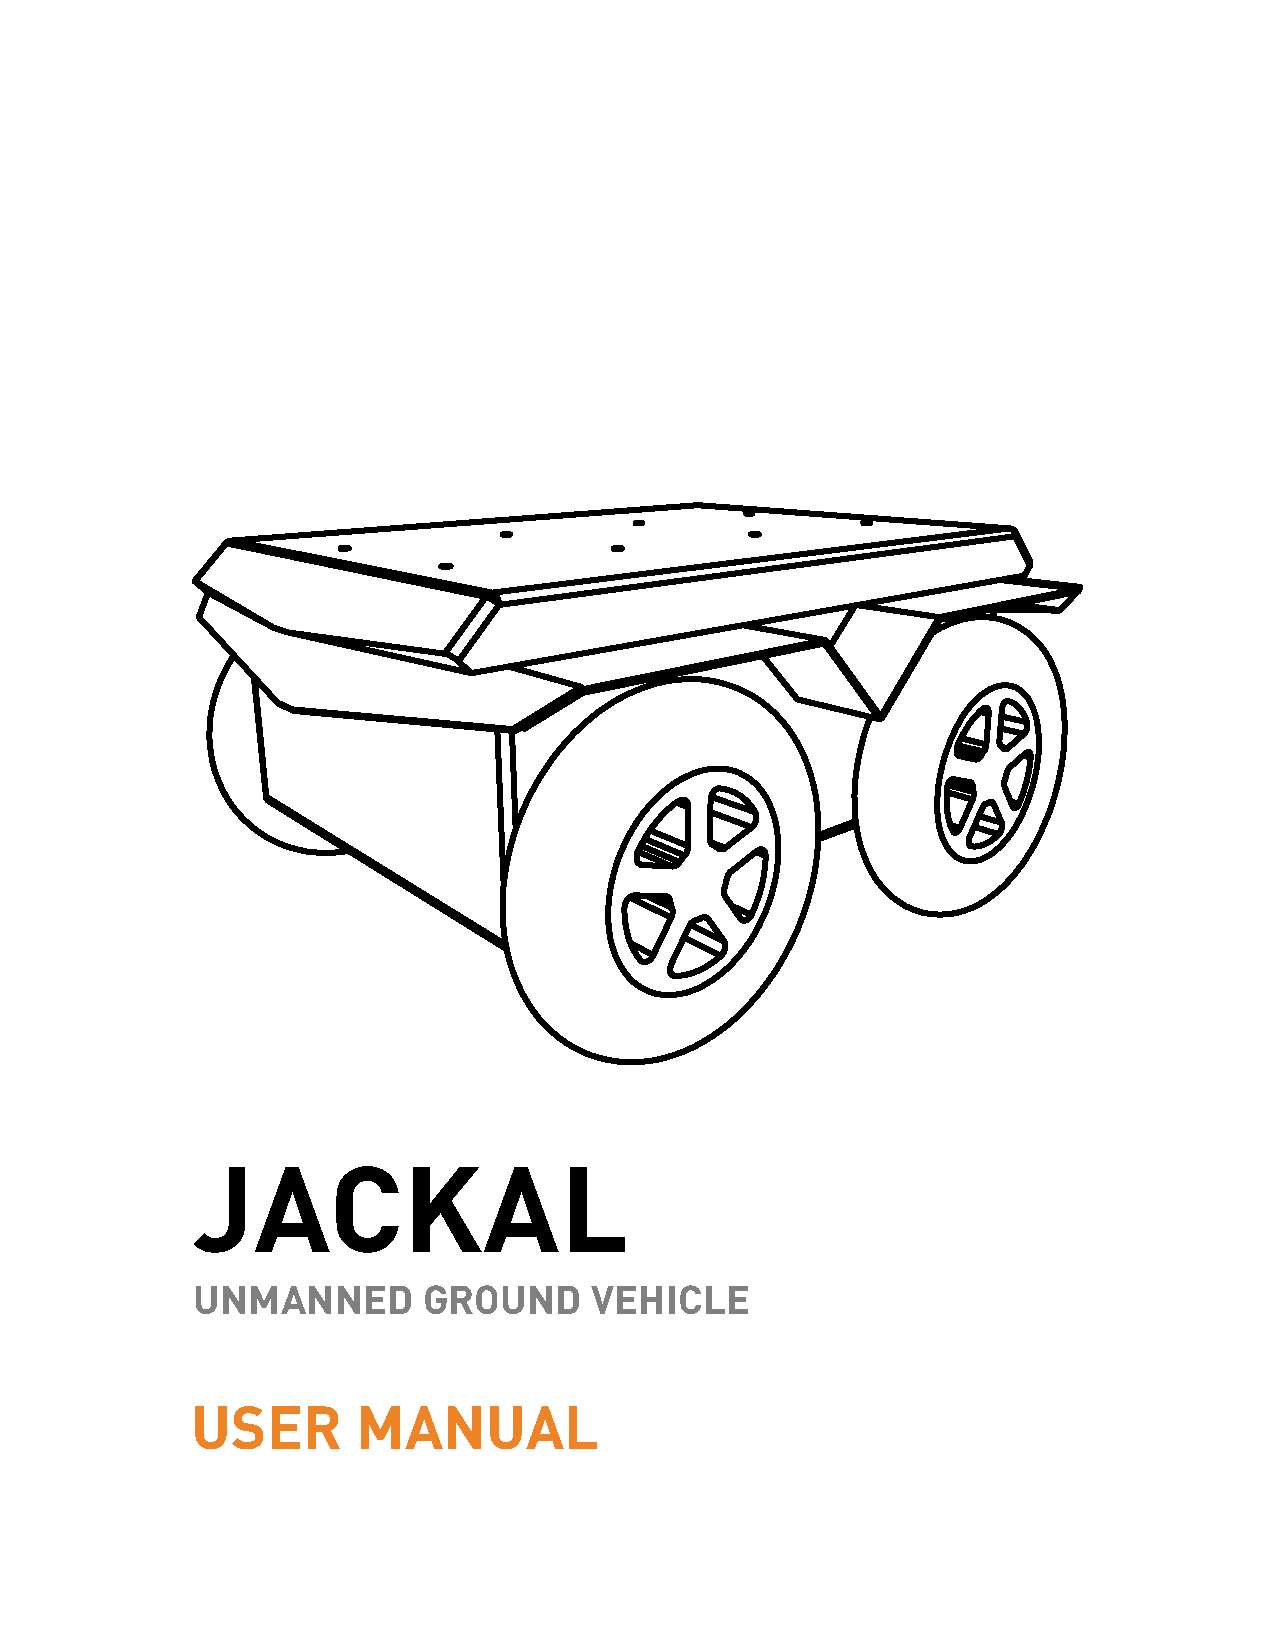
\includegraphics{gen/cover-page.pdf}
};
\end{tikzpicture}

\tableofcontents

\section{Introduction}

Jackal is a rugged, light, fast and easy-to-use unmanned ground vehicle for ROS Indigo, presented
by Clearpath Robotics.

Jackal includes as standard an internal x86 PC, as well as basic IMU and GPS. Standard perception
modules are available, including URDF and simulator integration, and demonstration applications.
Please inquire with Clearpath Robotics for details.

\subsection{What's Included}

Contained in your Jackal shipment are the following items:

\begin{itemize}
  \item Jackal UGV
  \item 270 watt-hour lithium battery pack
  \item 110V/220V universal charger
  \item Sony Bluetooth controller
\end{itemize}

If you elected to purchase standard upgrade modules, these will be integrated into your Jackal chassis.

\section{Getting Started}

The first step is to power up your Jackal and have some fun driving it around!

\subsection{Talking to Jackal}

The next thing you probably want to do is get Jackal on your wireless network.

\subsection{Jackal Desktop}

\begin{lstlisting}
sudo apt-get install ros-indigo-jackal-desktop
\end{lstlisting}


\end{document}
